\label{mean_comp}
In this part, the mean of each entry is compared to the mean of each other entry.
Let $H_{0}$ and $H_{1}$ denote the hypotheses:

\begin{displaymath}
  H_{0} : \mu_{ij} \ge \mu_{i'j} , \; H_{1} : \mu_{ij} < \mu_{i'j}.
\end{displaymath}

The difference $\mu_{ij}-\mu_{i'j}$ between the means of germplasm $i$ and population $i'$ in environment $j$ was considered as significant if either $H_{0}$ or $H_{1}$ had a high posterior probability, that is if $Pr\{H_{0}|y\} > 1 - \alpha$ or $Pr\{H_{1}|y\}> 1 - \alpha$, where
$\alpha$ was some specified threshold.
The difference was considered as not significant otherwise.
The posterior probability of a hypothesis was estimated by the proportion of MCMC simulations for
which this hypothesis was satisfied (Figure~\ref{proba}).

Groups are made based on the probabilites.
Germplasms which share the same group are not different.
Germplasms which do not share the same groupe are different.

The threshold $\alpha$ that depends on agronomic objectives.
This threshold is set by default to $\alpha=0.1/I$ (with $I$ the number of entries in a given environnement).
It corresponded to a `soft' Bonferroni correction, the Bonferroni correction being very conservative.

As one objective of this PPB programme is that farmers (re)learn selection, the threshold could be adjusted to allow the detection of at least two groups instead of having farmers choose at random.
The initial value could be set to $\alpha=0.1/I$ and if only one group is obtained, then this value could be adjusted to allow the detection of two groups.
In this cases, the farmers should be informed of the lower degree of confidence that there are significant differences among entries.

\begin{figure}[H]
\begin{center}
\begin{pspicture}(10,10)
\rput[bl](0,0){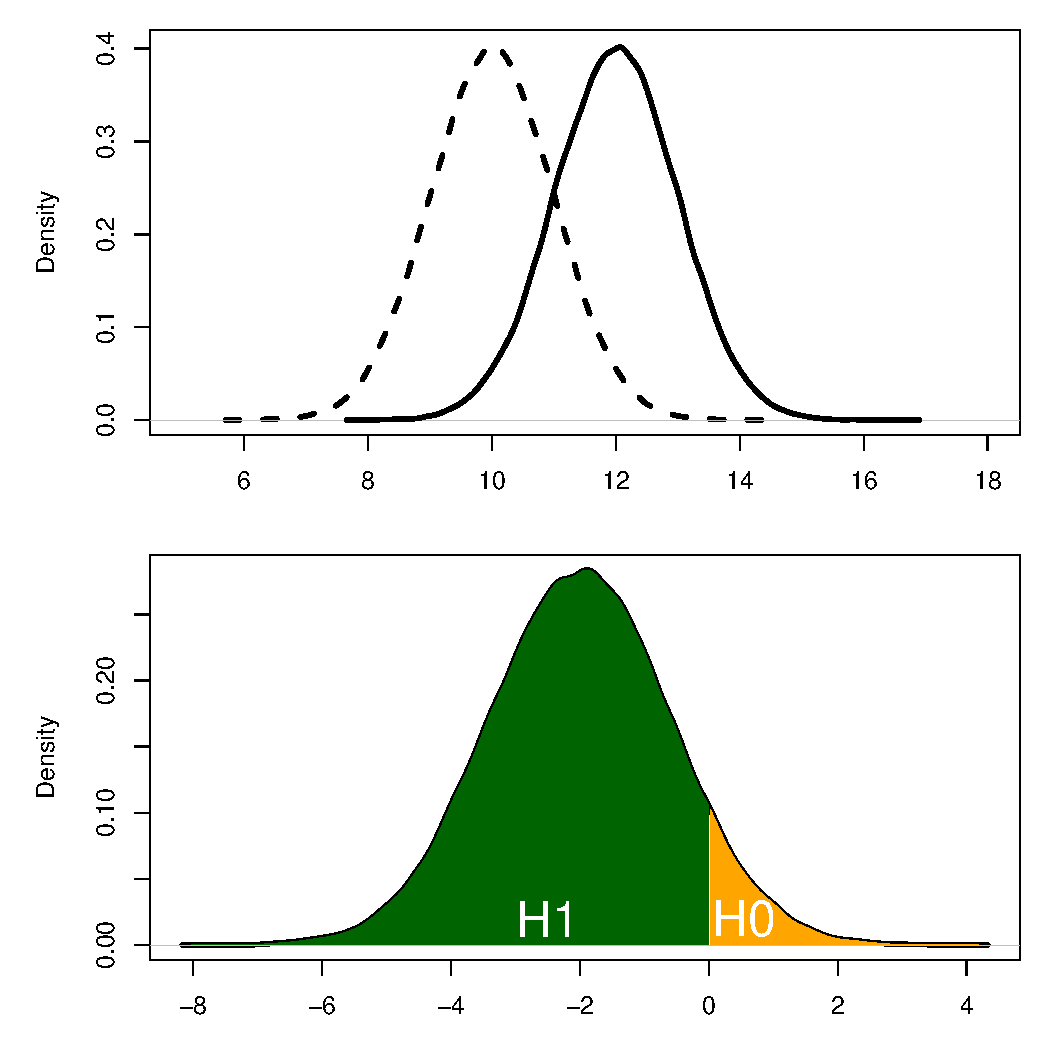
\includegraphics[width=.6\textwidth]{proba}}
\rput[b](3,7){$\mu_{ij}$}
\rput[b](7.5,7){$\mu_{i'j}$}
\rput[b](3,3){$\mu_{ij} - \mu_{i'j}$}
\end{pspicture}
\end{center}
\caption{Mean comparison between $\mu_{ij}$ (dash line) and $\mu_{i'j}$ (plain line).}
\label{proba}
\end{figure}

%% R code to get proba.pdf %%
%
%pdf("proba.pdf")
%
%par(mfrow=c(2,1),mar=c(3,5,1,1))
%
%a = rnorm(100000,10)
%d <- density(a)
%plot(d, type='l', xlab="", main="", xlim=c(5,18), lty=2, lwd=3)
%
%b = rnorm(100000,12)
%d <- density(b)
%lines(d,lty=1, lwd=3)
%
%diff = a - b
%
%d <- density(diff)
%plot(d, type='l', xlab="", main="", lty=1, lwd=3)
%
%toget = which(d$x>=0)
%H0x = d$x[toget]
%H0y = d$y[toget]
%
%toget = which(d$x<0)
%H1x = d$x[toget]
%H1y = d$y[toget]
%
%x <- H0x
%y <- H0y
%polygon( c(x,rev(x)), c(rep(0,length(x)),rev(y)), border=NA, col="orange" )
%
%x <- H1x
%y <- H1y
%polygon( c(x,rev(x)), c(rep(0,length(x)),rev(y)), border=NA, col="darkgreen" )
%
%text(-2.5,0.02,"H1", cex=2, col="white")
%text(0.55,0.02,"H0", cex=2, col="white")
%
%dev.off()



